\documentclass[11pt,a4paper]{ltjsarticle}
\usepackage{luatexja-fontspec}
\usepackage{geometry}
\usepackage{booktabs}
\usepackage{array}
\usepackage{enumitem}
\usepackage{graphicx}
\usepackage{hyperref}
\usepackage{xcolor}
\usepackage{amsmath}

\geometry{margin=24mm}

% 和文の太字（\textbf）は明朝に太字ウェイトが無いため，慣例どおり角ゴシックで表現する
\setmainjfont[BoldFont=Hiragino Kaku Gothic ProN]{Hiragino Mincho ProN}
\setsansjfont{Hiragino Kaku Gothic ProN}

\hypersetup{colorlinks=true, linkcolor=blue!60!black, urlcolor=blue!60!black}

\newcommand{\rkc}{\textrm{Recall@}K_{\textrm{correct}}}

\title{{\sffamily 進捗報告 v6（追補）：データベース拡大・難ケース追加・\\評価指標の精緻化による Set-aware GNN リランカーの頑健性検証}}
\author{宮村 和大}
\date{2026年6月2日}

\begin{document}
\maketitle

\noindent\textbf{本資料の位置づけ}：本資料は2026年5月18日提出の進捗報告 v5（以下「前回報告」）の\textbf{追補}である．前回報告と重複する手法・背景の説明は省き，新規結果に絞る．数値はすべて \texttt{experiments/} 配下の実験 JSON で確認した実測値であり，10 シード（\texttt{source\_id} 単位で訓練／評価を分割しリークを防止）で評価した．

%======================================================================
\section{前回報告（v5）からの変更点}
%======================================================================
\begin{itemize}[leftmargin=1.4em, nosep]
  \item \textbf{データを 3.4 倍に拡大}：収録数式 3{,}244 $\to$ \textbf{11{,}146式}，訓練ケース 1{,}107 $\to$ \textbf{2{,}838件}．うち微分代数方程式系（DAE）を模した\textbf{難ケースを 1{,}000 件}新規追加（図~\ref{fig:data}）．
  \item \textbf{主指標を $\rkc$ に変更}：天井で飽和する MRR\_first が隠していた差を可視化する指標（情報検索の R-precision と同義）を採用．
  \item \textbf{難ケースほど本手法の優位が拡大}：baseline との $\rkc$ 差は標準 $+0.127$ $\to$ DAE のみ $+0.217$（図~\ref{fig:gradient}）．改善は\textbf{複数式・多変数}のケースに集中する（図~\ref{fig:impact}a）．
  \item \textbf{仮説B（分野横断収集の要否）を再検定し結論を訂正}：v5 は MRR\_first で「差なし」としたが，$\rkc$ では\textbf{フル DB が有意に優れる}（$+0.048$，$p=0.044$；図~\ref{fig:impact}b）．加えて 13 通りのハイパーパラメータで頑健，外部の LLM 直接生成も上回る（図~\ref{fig:llm}）．
\end{itemize}

%======================================================================
\section{データセット：規模・内訳・難易度}\label{sec:data}
%======================================================================

データ規模と構成を図~\ref{fig:data}に示す．訓練ケースは 2{,}838 件，うち \textbf{74.6\%} が正解に 2 式以上を要する\textbf{複数式}ケースであり，「式を組合せとして選ぶ」本手法の主戦場となっている．

新規追加した DAE 難ケース（1{,}000 件，Anthropic Claude Sonnet 4.5 で生成）は，物理モデルとして典型的な「常微分方程式（ODE）＋付随する代数式」の連立を模す．生成手順は，(i) ODE を 1 本選んで正解集合の種とし，(ii) 同一文献内で\textbf{変数を共有}する式（速度式・物性式など）を正解集合に追加し，(iii) 正解式数が $X\in\{1,\dots,10\}$ に達するまで反復，(iv) 各式の代表変数を出力に加えて\textbf{自由度ゼロ}（入力数 $+$ 方程式数 $=$ 出力数 $+$ 既知数）を構成上保証する，というものである．たとえば連続槽型反応器（CSTR）で槽内濃度 $C_A(t)$ と反応速度 $r_A$ を求める問題は，物質収支 ODE $V\,dC_A/dt = F(C_{A0}-C_A)-V r_A$ と Arrhenius 速度式 $r_A=k\,C_A,\ k=A\exp(-E/RT)$ を\textbf{組合せて}初めて解ける．

\begin{figure}[htbp]
\centering
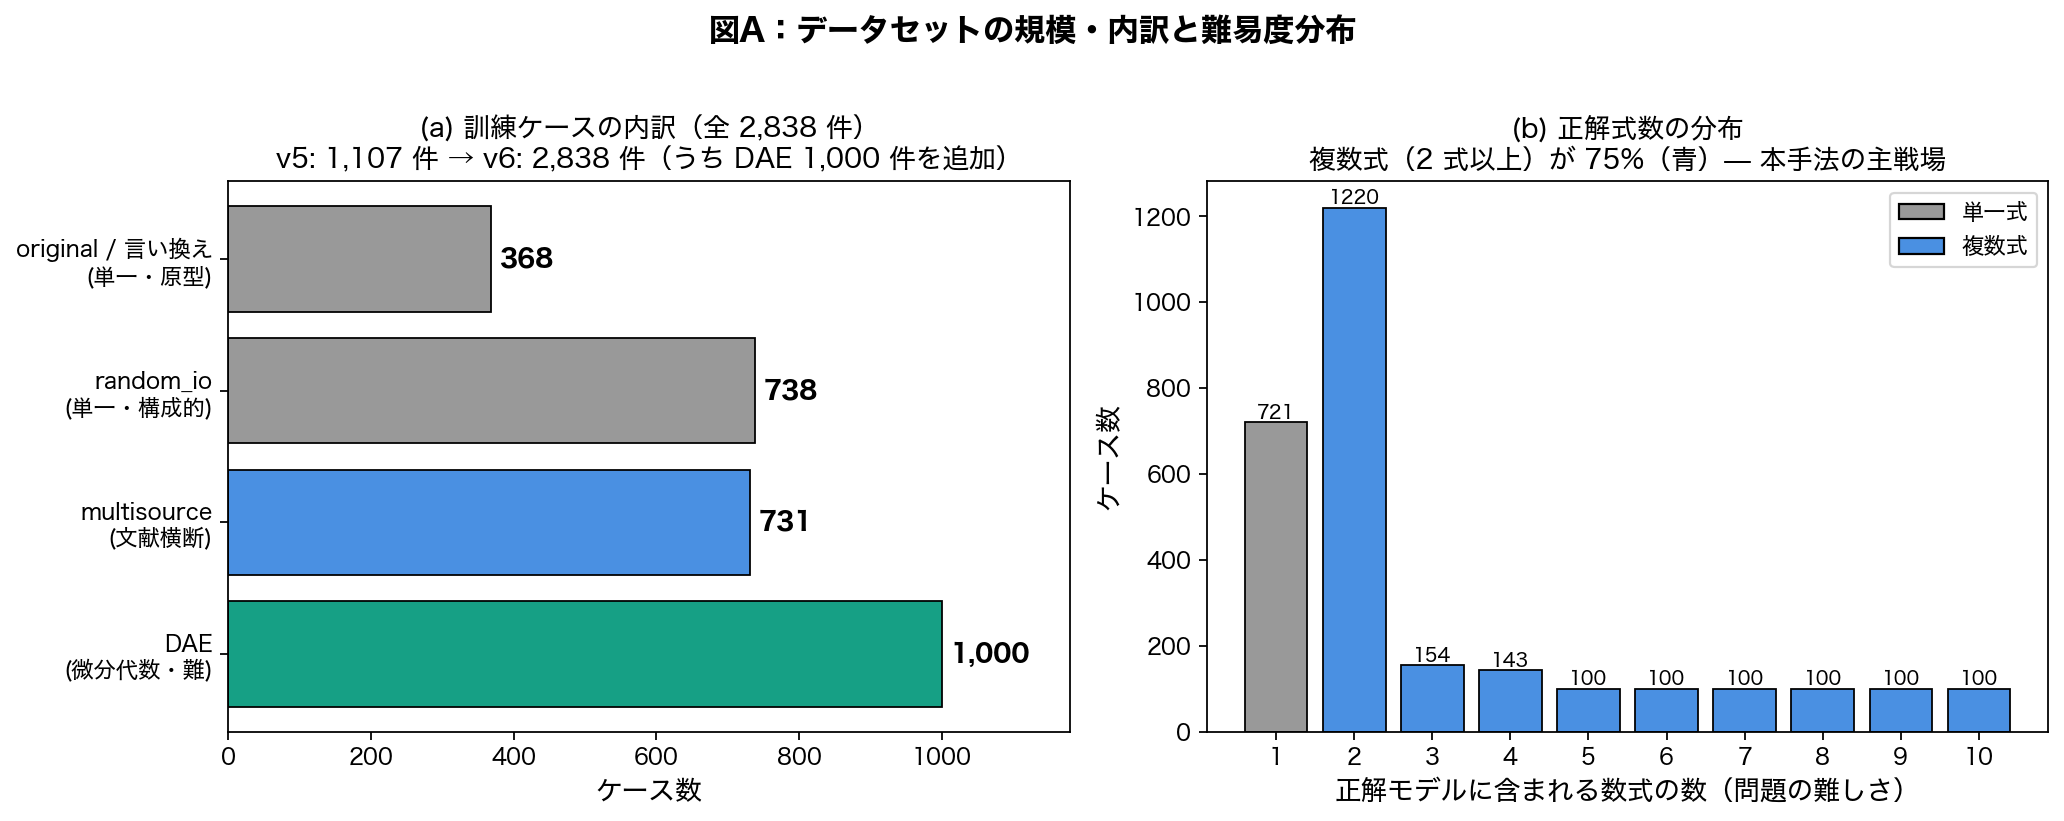
\includegraphics[width=\linewidth]{figures/fig_v6_dataset.png}
\caption{データセットの規模・内訳と難易度分布．(a) 訓練ケース 2{,}838 件の variant 別構成（DAE 1{,}000 件を新規追加，緑）．(b) 正解式数の分布：複数式（2 式以上，青）が全体の 74.6\%．}
\label{fig:data}
\end{figure}

%======================================================================
\section{評価指標 $\rkc$ の導入}\label{sec:metric}
%======================================================================

従来の主指標 MRR\_first（最初に当たった正解の順位の逆数）は，正解が 1 件でも上位に来れば 1.0 に近づくため，複数式を揃える能力を測れず，天井付近で飽和して手法間の差を覆い隠す．本版では，正解式が $n_{\textrm{correct}}$ 件あるとき\textbf{上位 $K=n_{\textrm{correct}}$ 件}の正解割合 $\rkc=|\textrm{Top-}K\cap\mathcal{R}_q|/|\mathcal{R}_q|$（$\mathcal{R}_q$ は正解集合，情報検索の R-precision と同義）を主指標とする．「\textbf{必要な式をちょうどその本数だけ上位に並べられたか}」を直接測り，飽和しにくい．補助指標として MAP（平均適合率），MRR\_first も併記する．

%======================================================================
\section{実験結果}
%======================================================================

\subsection{難易度勾配：難ケースほど優位が拡大}\label{sec:gradient}

評価集合に占める難ケースの比率を 3 段階に変えて baseline（古典 IR，Stage~1）と reranker-10S（Set-aware 特徴量を含む Stage~2）を比較した（図~\ref{fig:gradient}）．\textbf{古典 IR は難ケースが増えると $\rkc$ が $0.79\to0.48$ へ急落するのに対し，本手法は $0.91\to0.70$ と緩やかにしか落ちず}，両者の差は $+0.127\to+0.210\to+0.217$ と単調に拡大する．数式グラフ上で式を組合せとして評価する本手法の発想が，難しい組合せ問題でこそ効くことを示す．

\begin{figure}[htbp]
\centering
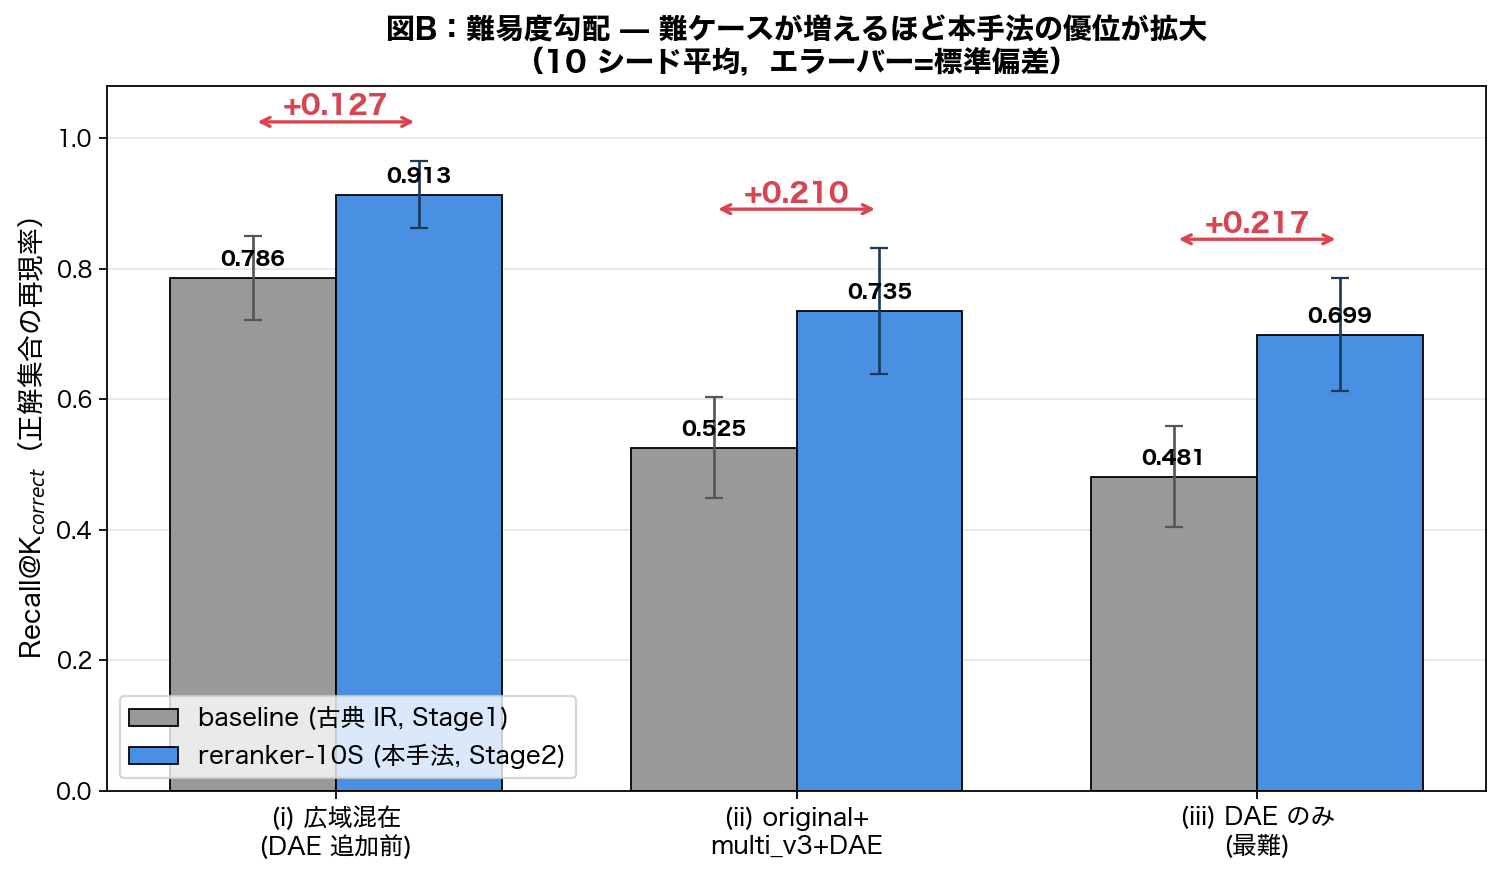
\includegraphics[width=0.82\linewidth]{figures/fig_v6_gradient.png}
\caption{難ケース比率の異なる 3 設定における $\rkc$（10 シード平均，エラーバー＝標準偏差）．難ケースが増えるほど baseline は低下し，本手法との差（赤）が拡大する．}
\label{fig:gradient}
\end{figure}

\subsection{本手法はどこで効くか／なぜ指標を変えたか}\label{sec:impact}

図~\ref{fig:impact}(a) は正解式数別の $\rkc$ である．\textbf{単一式では baseline が既に高く本手法の上乗せはほぼ無い}（$+0.02$）が，\textbf{複数式では $+0.21\sim0.26$ の大幅改善}を示す．入力変数が多い（11 以上）ケースでも同様に $+0.245$ 改善する．本手法は「易しい問題を壊さず，難しい組合せ問題で効く」という望ましい振舞いを持つ．

図~\ref{fig:impact}(b) は，加納先生のご指摘「\textbf{分野横断的に収集する必要はない}」（仮説B）の再検定である．v5 は MRR\_first がフル DB と化学工学限定 DB でほぼ同じ（差 $+0.003$）であったため「DB 規模の影響なし」としていた．しかし飽和しない $\rkc$ では\textbf{フル DB（11{,}146式・全分野）が限定 DB を有意に上回る}（$0.923$ vs $0.875$，差 $+0.048$，対応のある $t$ 検定 $p=0.044$，Wilcoxon $p=0.037$，効果量 Cohen's $d=0.74$ 中程度）．すなわち v5 の暫定結論は\textbf{指標選択の副作用}であり，広く集める方針の妥当性が支持された（ただし差は中程度で，限定 DB でも $\rkc=0.87$ の実用水準には達する）．

\begin{figure}[htbp]
\centering
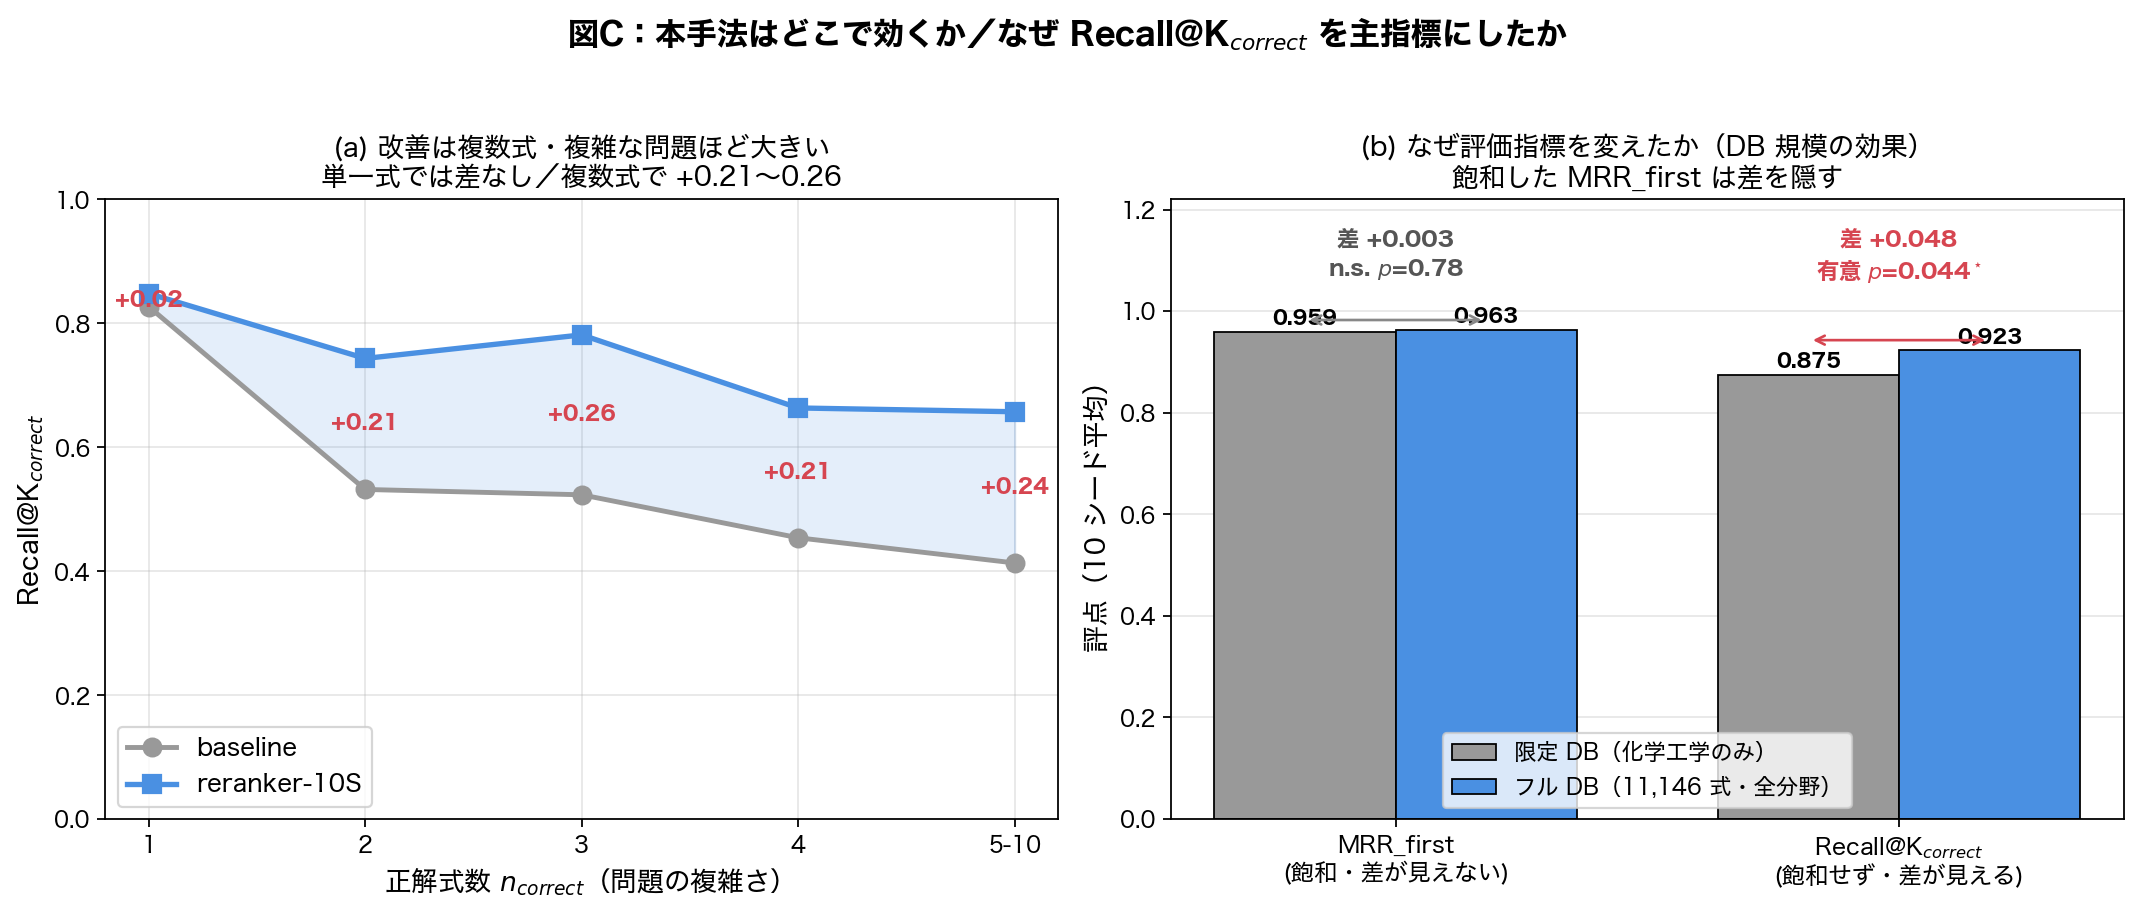
\includegraphics[width=\linewidth]{figures/fig_v6_impact.png}
\caption{(a) 正解式数別の $\rkc$：改善は複数式・複雑な問題ほど大きい．(b) 仮説B の再検定：飽和した MRR\_first では差が見えないが，$\rkc$ ではフル DB が有意に優位（$p=0.044$）．}
\label{fig:impact}
\end{figure}

\subsection{ハイパーパラメータ頑健性}\label{sec:robust}

「本手法の優位は脆弱なチューニングの産物では」という査読上の懸念に対し，学習率（$10^{-4}$--$10^{-2}$），隠れ層次元（64/128/256），epoch（20/40），margin（0.1/0.3）を振った 13 設定で $\rkc$ を測った．\textbf{全 13 設定が $0.732$--$0.742$ の狭い範囲に収まり，設定間レンジ $0.0094$ はシード間標準偏差（約 $0.097$）の約 $1/10$}にすぎない．本手法の強さは特定のチューニングに依存せず頑健である．

\subsection{外部ベースライン：LLM 直接生成との同一条件比較}\label{sec:llm}

「LLM で直接解けるなら本手法は不要では」という加藤先生のご指摘に答えるため，大規模言語モデル（Claude，Sonnet 系）を\textbf{問題を解く側}として用い，背景文と入出力変数のみから数式を生成させて現行 11{,}146式 DB と照合した（本研究で LLM を使うのはケース生成のみで，検索タスクには使わない）．比較対象の baseline・reranker-10S も同一サブセット・同一 DB で再評価した（リーク防止のため対象ケースをテスト分割でのみ評価）．

結果を図~\ref{fig:llm}に示す．\textbf{易しい単一ソースでは検索系（両 Stage）が LLM を圧倒}する（$\rkc$ で baseline $0.982$／reranker $0.975$ vs LLM $0.707$）．一方\textbf{難しい複数ソースでは，古典 IR 単独は LLM を下回る}（$0.575<0.842$）が，\textbf{reranker-10S は baseline を $+0.367$ 改善して LLM をも上回る}（$0.942$）．文章類似度だけでは複数文献の式を組合せられず，Set-aware リランカーが本質的に必要であることを同一条件で実証した．なお本比較は単一 29 件・複数 20 件の小規模・held-out 評価（1 ケースあたり平均約 1--2 シード）であり，傾向の確認と位置づける．

\begin{figure}[htbp]
\centering
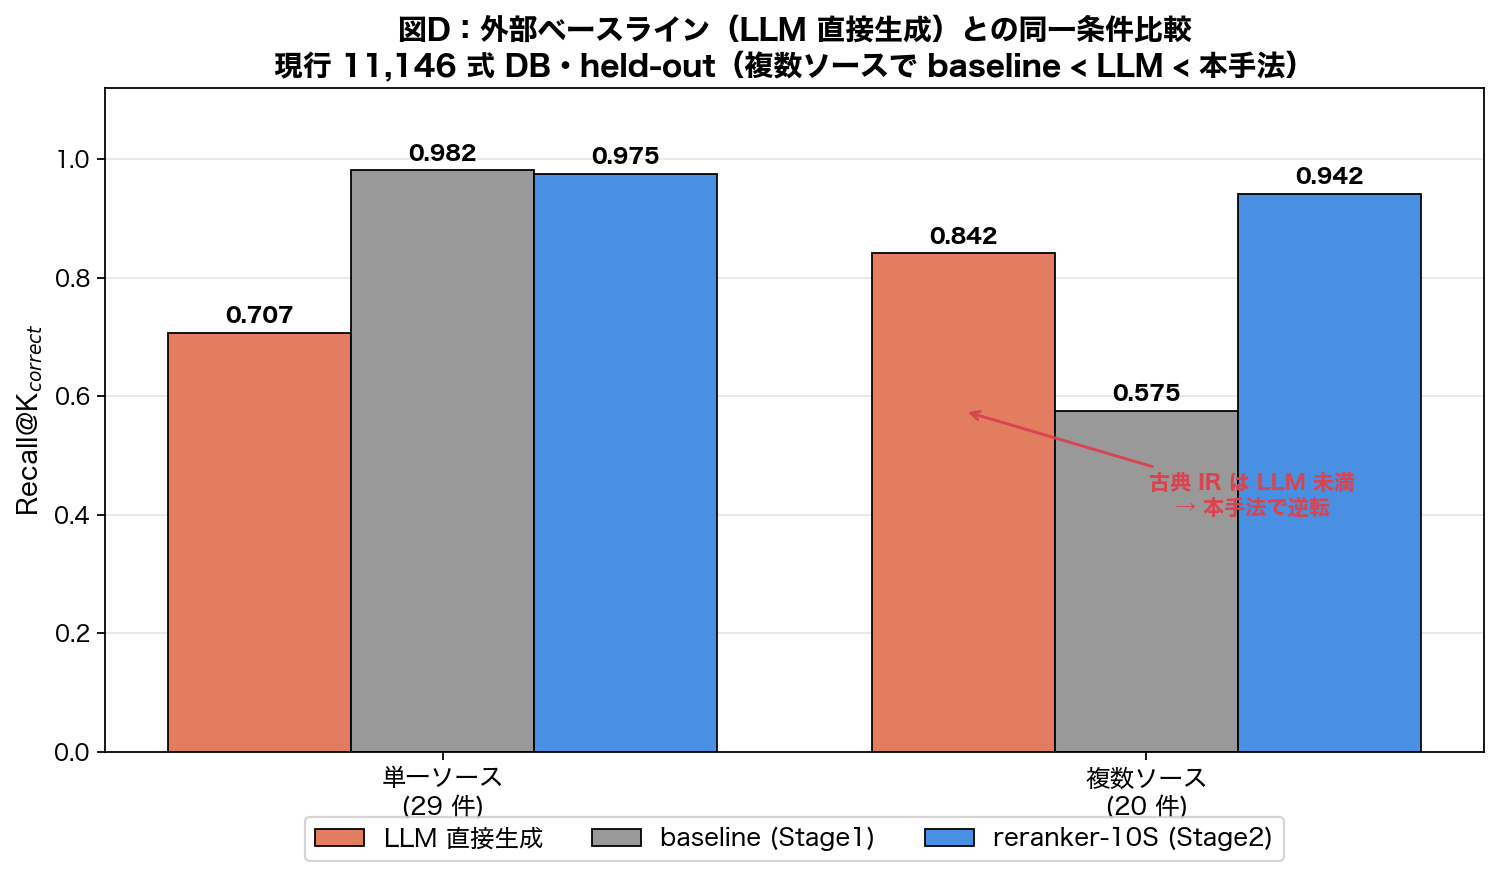
\includegraphics[width=0.82\linewidth]{figures/fig_v6_llm.png}
\caption{LLM 直接生成 vs baseline(Stage1) vs reranker-10S(Stage2) の同一条件比較（$\rkc$，現行 11{,}146式 DB）．複数ソースで baseline $<$ LLM $<$ 本手法．}
\label{fig:llm}
\end{figure}

%======================================================================
\section{考察と今後の方針}
%======================================================================
\begin{itemize}[leftmargin=1.4em, nosep]
  \item \textbf{なぜ効くか}：DAE・複数式・多変数のケースは単独式の文章類似度では絞れず，式どうしの\textbf{変数共有（補完性・一貫性）}という構造情報が効く．易しい問題は baseline が天井のため上乗せは小さい（図~\ref{fig:impact}a）．
  \item \textbf{指標の重要性}：MRR\_first の飽和は DB 規模の効果（仮説B）も改善幅も隠していた．$\rkc$ への切替で初めて両者が可視化された．
  \item \textbf{頑健性と外部比較}：13 設定で差が出ないことは優位が\textbf{構造的特徴量そのもの}に由来することを，LLM との同一条件比較は\textbf{古典 IR では足りず本手法が必要}であることを示す．
  \item \textbf{今後}：(1) 修論・論文「Set-aware graph features for multi-equation physical model retrieval」の執筆，(2) LLM 外部比較の標本拡充（難ケースでの LLM 評価），(3) Set-aware 特徴量の拡張（listwise 学習・hard negative），(4) 変数記述の意味類似度による表記揺れの学習的吸収．
\end{itemize}

%======================================================================
\section{まとめ}
%======================================================================
データベースを 11{,}146 式・2{,}838 ケースに拡大し DAE 難ケースで難易度勾配を作ったところ，\textbf{難しい問題ほど Set-aware リランカーの優位（$\rkc$）が $+0.13\to+0.22$ と拡大}した．飽和しない $\rkc$ により分野横断収集の効果（仮説B，$+0.048$，$p=0.044$）が新たに有意と判明し v5 の暫定結論を訂正，ハイパーパラメータにも頑健で，外部の LLM 直接生成を複数ソースで上回ることを同一条件で確認した．

\end{document}
